
\documentclass[12pt,a4paper]{report}
\usepackage[utf8]{inputenc}
\usepackage{amsmath}
\usepackage{amsfonts}
\usepackage{amssymb}
\usepackage{graphicx}
\usepackage{enumitem}
\usepackage[left=2cm, right=2cm, top=4cm, bottom=2cm]{geometry}

\begin{document}
	%Portada
	\begin{titlepage}
		\centering
		{\scshape\LARGE Universidad Nacional Autónoma de México \par}
		\vspace{1cm}
		{\scshape\Large Probabilidad I\par}
		\vspace{1.5cm}
		{\huge\bfseries Tarea V\par}
		\vspace{.5cm}

		{\Large\itshape Alan Ernesto Arteaga Vázquez \par}
		 \vspace{.5cm}
		{\Large\itshape Raúl Llamosas Alvarado \par}
		 \vspace{.5cm}
		{\Large\itshape Edgar Quiroz Castañeda \par}
	    \vspace{.5cm}
		{\Large\itshape Jean Paul Ruiz Melo\par}
		\vspace{.5cm}
		{\Large\itshape Sandra Del Mar Soto Corderi \par}

		\vfill
		 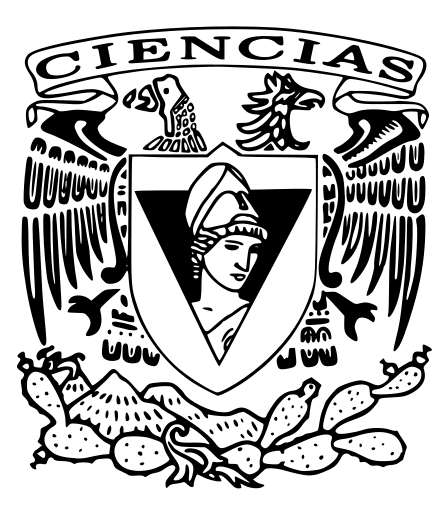
\includegraphics[width=0.5\textwidth]{escudo.png}
		\vfill

		{\large Lunes 26 de octubre del 2018 \par}
	\end{titlepage}

	\pagebreak
	\setlength{\voffset}{-0.75in}
	\setlength{\headsep}{5pt}

	%Ejericios
	\begin{enumerate}
		%1
		\item{
			Suponga de Gage e Itzel participan en un juego, el cual consiste en
			lanzar un dado hasta que alguno de los dos obtenga un 6. Suponga
			que Itzel es la primera en lanzar un dado. ¿Cuál es la probabilidad
			de que Gage gane?
			\\ \\
	        Tenemos que la probabilidad de que gane Gage en su primer lanzamiento es la
		probabilidad de que lanzo un 6 por la probabilidad de que Itzel no lanzo un
		6, lo cual es:
	        \[\frac{1}{6}\frac{5}{6}\]
	        De esto, tenemos que en su tercer lanzamiento es la probabilidad de que en
		ninguno de los anteriors lanzo un 	6 por la probabilidad que lanzo  un 6:
	        \[\frac{1}{6}\frac{5}{6}\frac{5}{6}\frac{5}{6}\]
	        Y esto lo podemos ver como:
	        \[\frac{1}{6}(\frac{5}{6})^{3}\]
	        Entonces en el n-esimo lanzamiento tendremos:
	        \[\frac{1}{6}(\frac{5}{6})^{n}\]

	        Por lo tanto la probabilidad de que Gage gane es:
	        \[\frac{1}{6}\frac{5}{6} + \frac{1}{6}(\frac{5}{6})^{3} + ... + \frac{1}{6}(\frac{5}{6})^{n}\]

	        \[\sum^{\infty}_{x=1} \frac{1}{6}(\frac{5}{6})^{2x - 1}\]


	       `

		}
		%2
		\item{
			Considere una variable aleatoria $X$ con una función de densidad
			\[
				f_X(x) = \begin{cases}
					\frac{1-|\frac{x-\alpha}{\beta}|}{\beta},
					$ si $ x \in (\alpha - \beta, \alpha + \beta)\\
					0, $ en otro caso$
				\end{cases}
			\]
			Prueve que $f_X(x)$ es de densidad. Grafíquela.\\

			Podemos ver a $x - \alpha$ como u, entonces:
			\[\alpha - \beta - \alpha = -\beta\]
			\[\beta - \alpha - \alpha = \beta\]
			Estos van a ser los limites inferiores y superiores del integral:
    			\[\int^\beta_{-\beta}  \frac{1-|\frac{u}{\beta}|}{\beta}du\]
			Pero es valor absoluto entonces:
			\[\int^\beta_{-\beta} \frac{1}{\beta}du - \int^\beta_{-\beta} \frac{|\frac{u}{\beta}|}{\beta}du\]
			\[\int^\beta_{-\beta} \frac{1}{\beta}du -( \int^\beta_{0} \frac{\frac{u}{\beta}}{\beta}du + 				\int^0_{-\beta}  \frac{\frac{u}{\beta}}{\beta}du)\]
			\[(\frac{\beta}{\beta}-\frac{-\beta}{\beta}) - ((\frac{\beta^2}{2\beta^2} - 0)
			+ (0 - \frac{(-\beta)^2}{2\beta^2}))\]
			\[(1-(-1) - (\frac{1}{2} + \frac{1}{2})\]
			\[2-1\]
			\[1\]
			Entonces $f_X(x)$ es de densidad.\\
			En la grafica tendremos un v invertido. Donde $\beta$ define que tan grande es su angulo,
			si $\beta$ es grande, el angulo sera menor. Ademas, el punto de origen se define a
			respeto de $\beta$ y $\alpha$. El mas pequeno que es $\beta$, mas grande es y, y $x$
			= $\alpha$.
		}

		%3
		\item{
			\textit{(La paradoja de San Petersburgo, planteada por Nicolás
			Bernoulli en 1728)}.\\
			De acuerdo a la historia, en casino de SanPetersburgo estaba
			dispuesto a ofrecer cualquier tipo de juego siempre que la
			dirección del casino pudiera establecer el precio de la entrara
			que se paga por participar. Se propone el siguiente juego: suponga
			que alguien lanza una moneda balanceada y se reciben $2^n$ pesos
			si cae cara en el $n-$ésimo lanzamiento.\\
			Sea $X$ la ganancia del jugador.
			\begin{enumerate}
				%a
				\item {
				Calcule $\mathbb{E}(X)$.

				Tenemos que en el primer lanzamiento es:
				\[\frac{1}{2}2^{1}\]
				En el segundo es:
				\[(\frac{1}{2})(\frac{1}{2})2^{2} = \frac{1}{4}4\]
				Y asi se va hasta n:
				\[(\frac{1}{2})^{n} = \frac{1}{2^{n}}2^{n}\]
				}
				De donde $\mathbb{E}(X)$ es:
				\[\mathbb{E}(X) = \frac{1}{2}2 + \frac{1}{4}4 + ... +  \frac{1}{2^{n}}2^{n}\]
				\[= 1 + 1 + ... + 1\]
				Como puede ser cualquier numero de lanzamientos:
				\[= \infty\]

				%b
				\item {
				¿Estaría dispuesto a liquidar toda la fortuna material que
				posee a cambio de la entrada de este juego?\\
				No, porque de todas formas es menos probable que ganas lo suficiente para que vale la pena.
				}
			\end{enumerate}
		}

		%4
		\item{
			Suponga que se lanzan $n$ dados. Sea $S_n$ la suma de las caras
			obtenidaas al lanzar los $n$ dados.
			\begin{enumerate}
				%a
				\item {
					Encuentre $\mathbb{E}(S_2)$\\
					La esperanza de solo un dado seria:
					\[(\frac{1}{6})1 + (\frac{1}{6})2 + (\frac{1}{6})3 + (\frac{1}{6})4 + (\frac{1}{6})5 + (\frac{1}{6})6\]
					Entonces para dos seria:
					\[\mathbb{E}(S_2) = 2((\frac{1}{6})1 + (\frac{1}{6})2 + (\frac{1}{6})3 + (\frac{1}{6})4 + (\frac{1}{6})5 + (\frac{1}{6})6))\]
					\[= 2(\frac{1+2+3+4+5+6}{6})\]
					\[=\frac{42}{6} = \frac{6 * 7}{6}\]
					\[\mathbb{E}(S_2) = 7\]
				}

				%b
				\item {
					Encuentre $\mathbb{E}(S_n)$\\
					Entonces tenemos lo mismo que el inciso a, solo que en lugar de 2 dados, son n:
					\[\mathbb{E}(S_n) = n((\frac{1}{6}) + (\frac{2}{6}) + (\frac{3}{6})+ (\frac{4}{6}) + (\frac{5}{6}) + (\frac{6}{6}))\]
					\[= n(\frac{1+2+3+4+5+6}{6})\]
					\[= n(\frac{21}{6})\]
					\[= n(\frac{3 * 7}{6}) = n\frac{7}{2}\]
					De donde tenemos que:
					\[\mathbb{E}(S_n) = n(3.5)\]
				}
			\end{enumerate}
		}

		%5
		\item{
			Sea $Y$ una variable aleatoria con media $\mu > 0$ y varianza
			$\sigma^2 > 0$. Para que valor de $a > 0$ se minimiza
			\begin{enumerate}
				%a
				\item {
					$\mathbb{E}((Y-a)^n)$
				}
				\newline
				Consideremos a $g(a)$ una función de $"a"$, tal que
					$$ g(a) = \mathbb{E}((Y - a)^2) $$
				desarrollando, se sigue:
					$$ \mathbb{E}((Y - a)^2) = \mathbb{E}(Y^2 - 2aY + a^2) $$
				luego, por propiedades de la esperanza:
					$$ g(a) = \mathbb{E}(Y^2) - 2a\mathbb{E}(Y) + a^2 $$
				ahora, para encontrar el valor de a que minimiza a $ g(a) $, se
				tiene derivando:
					$$ \frac{d}{da} [\mathbb{E}(Y^2) - 2a\mathbb{E}(Y) + a^2]
					 = -2\mathbb{E}(Y) + 2a $$
				luego, igualando a cero la derivada:
					$$ 0  =-2\mathbb{E}(Y) + 2a $$
					$$ a = \mathbb{E}(Y) $$
				así, se tiene que a se minimiza cuando $ a = \mathbb{E}(Y) $,
				ahora, solo resta corroborar que en punto es un mínimo, así,
				usando el criterio de la segunda derivada:
					$$ \frac{d^2}{da^2}[\mathbb{E}(Y^2) - 2a\mathbb{E}(Y) + a^2]
				     = 2$$
				y evaluando el punto crítico en la segunda derivada, se tiene:
					$$ f''(\mathbb{E}(Y)) = 2 $$
				así, como la evaluación en la segunda derivada es positiva, se sigue que $ \mathbb{E}(Y) = a $ minimiza a $"g(a)"$.

				%b
				\item {
					$\mathbb{E}((aY-\frac{1}{a})^2)$
				}
				\newline
				Ahora, considerando a $ h(a) $ una función tal que
					$$ h(a) = \mathbb{E}((aY - \frac{1}{a})^2) $$
				desarrollando, se tiene:
					$$ \mathbb{E}((aY - \frac{1}{a})^2) = \mathbb{E}(a^2Y^2
					 - 2Y + \frac{1}{a^2}) $$
				entonces, por propiedades de la esperanza, se sigue:
					$$ h(a) = a^2\mathbb{E}(Y^2) - 2\mathbb{E}(y)
					 + \frac{1}{a^2} $$
			 	ahora, para encontrar el valor de a que minimiza a $ g(a) $, se
			 	tiene derivando:
			 		$$ \frac{d}{da} [a^2\mathbb{E}(Y^2) - 2\mathbb{E}(y)
					 + \frac{1}{a^2}]
			 	 	 = 2a\mathbb{E}(Y^2) - \frac{2}{a^3} $$
				igualando a cero:
					$$ 0 = 2a\mathbb{E}(Y^2) - \frac{2}{a^3} $$
					$$ \frac{2}{a^3} = 2a\mathbb{E}(Y^2) $$
					$$ \frac{1}{a^4} = \mathbb{E}(Y^2) $$
					$$ a^4 = \frac{1}{\mathbb{E}(Y^2) }$$
					$$ a = \sqrt[4]{ \frac{1}{\mathbb{E}(Y^2) }}$$
				finalmente, comprobamos que el punto $ a = \sqrt[4]{
				\frac{1}{\mathbb{E}(Y^2) }} $ es un mínimo aplicando el criterio
				de la segunda derivada, así:
					$$ \frac{d^2}{da^2}[a^2\mathbb{E}(Y^2) - 2\mathbb{E}(y)
					 + \frac{1}{a^2}] = 2\mathbb{E}(Y^2) + \frac{6}{a^4}$$
				evaluando en el punto crítico:
				    $$ f''\Big( \sqrt[4]{\frac{1}{\mathbb{E}(Y^2)}} \Big)
					 = 2\mathbb{E}(Y^2) + \frac{6}{\frac{1}{\mathbb{E}(Y^2)}}
					 = 2\mathbb{E}(Y^2) + 6\mathbb{E}(Y^2)$$
				ahora, como por hipótesis se tiene $ \mathbb{E}(Y) = \mu > 0 $ y
				$ Var(Y) = \sigma^2 > 0$, y por definición de varianza:
					$$ Var(Y) = \mathbb{E}(Y^2) - \mathbb{E}(Y)^2$$
					$$ \mathbb{E}(Y^2) = Var(Y) + \mathbb{E}(Y)^2$$
				entonces se tiene que $ \mathbb{E}(Y^2) > 0 $, por lo que
				también $ 8\mathbb{E}(Y^2) > 0 $, por lo que la evaluación de la
				segunda derivada en el punto es positiva, y por lo tanto, el
				punto $ a = \sqrt[4]{ \frac{1}{\mathbb{E}(Y^2) }} $ minimiza a
				$h(a)$.
			\end{enumerate}
		}

		%6
		\item{
			Sea $X$ una variable aleatoria con función de densidad
			\[f_X(x) = c \Big(\frac{1}{6}\Big)^x \mathbb{I}_{\mathbb{N}}(x)\]
			\begin{enumerate}
				%a
				\item {
					Determinar el valor de $c$ para que $f_X$ sea función de
					densidad.
				}
				\newline
				Para que $f_X^{(x)}$ cumpla ser función de densidad, debe
				ocurrir (ya que X es una variable aleatoria discreta):
					$$ 1 = \sum_{x = 1}^{\infty} c\Big(\frac{1}{6}\Big)^x $$
					$$ 1 = c \sum_{x = 1}^{\infty} \Big(\frac{1}{6}\Big)^x $$
				luego, como $ \Big( \frac{1}{6} \Big) < 1$, la serie converge de
				tal forma que:
					$$ 1 = c \Big(\frac{1}{1 - \frac{1}{6} }\Big)  $$
					$$ 1 = c \Big( \frac{1}{\frac{5}{6}} \Big)  $$
				se sigue entonces:
					$$ \frac{5}{6} = c $$

				%b
				\item {
					Encontrar la función generador de momentos $m_X(t)$.
				}
				\newline
				Se tiene que la función generadora de momentos para una variable
				aleatoria discreta puede ser hallada mediante:
					$$ m_X(t) = \sum_{j = 1}^{\infty} e^{tx_j} f_X^{(x_j)} $$
				aplicando la definición a la función de densidad dada:
					$$  m_X(t)
					 = \sum_{j = 1}^{\infty} e^{tx_j} \Big( \frac{5}{6} \Big)
					   \Big(\frac{1}{6}\Big)^{x_j}
					 = \Big( \frac{5}{6} \Big) \sum_{j = 1}^{\infty} e^{tx_j}
					   \Big(\frac{1}{6}\Big)^{x_j} $$
					$$ = \Big( \frac{5}{6} \Big) \sum_{j = 1}^{\infty}
					     \Big(\frac{e^t}{6}\Big)^{x_j} $$
				ahora, condicionando a $ \frac{e^t}{6} < 1 $, i.e. $ t < ln(6) $
				de tal forma que la serie converja, se tiene:
					$$ \Big( \frac{5}{6} \Big) \sum_{j = 1}^{\infty}
					     \Big(\frac{e^t}{6}\Big)^{x_j}
					 = \Big( \frac{5}{6} \Big)
					   \Big( \frac{1}{ 1 - \frac{e^t}{6}} \Big)
					 = \frac{\frac{5}{6}}{ 1 - \frac{e^t}{6}}$$
			\end{enumerate}
		}

		%7
		\item{
			Sea $X$ una función de densidad de probabilidad dada por
			\[f_X(x) = \frac{2}{3^x} \mathbb{I}_{\{1, 2, 3, ...\}}(x)\]
			¿Cuál es la probabilidad de que $X$ sea par?
		}
		\newline
		Se tiene que la probabilidad de que $X$ sea par, está dada por
			$$ P(X = 2) + P(X = 4) + P(X = 6) + ... + P(X = 2x) \text{ con }
			   x \in \{1,2,3, ...\} $$
		exprasándola en términos de la función de densidad:
			$$ f_X^{(2)} + f_X^{(4)} + f_X^{(6)} + ... + f_X^{(2x)} \text{ con }
			   x \in \{1,2,3, ...\} $$
		lo cual, también se puede expresar como :
			$$ \sum_{x = 1}^{\infty} f_X^{(2x)} $$
		que a su vez, es equivalente a :
			$$ \sum_{x = 1}^{\infty} \frac{2}{3^{2x}} $$
		desarrollando, tenemos:
			$$ \sum_{x = 1}^{\infty} \frac{2}{3^{2x}}
			 = \sum_{x = 1}^{\infty} 2 \frac{1}{3^{2x}}
			 = 2 \sum_{x = 1}^{\infty} \frac{1}{9^x}
			 = 2 \sum_{x = 1}^{\infty} \Big( \frac{1}{9} \Big)^x $$
		luego, sumando y restando $ \Big( \frac{1}{9} \Big)^0  $ de tal forma
		que el resultado no se vea alterado:
			$$ = 2 \Big[ \sum_{x = 1}^{\infty} \Big( \frac{1}{9} \Big)^x
			   + \Big( \frac{1}{9} \Big)^0 - \Big( \frac{1}{9} \Big)^0 \Big] $$
			$$ = 2 \Big[  \sum_{x = 0}^{\infty} \Big( \frac{1}{9} \Big)^x
			   - \Big( \frac{1}{9} \Big)^0 \Big] $$
			$$ = 2 \Big[ \sum_{x = 0}^{\infty} \Big( \frac{1}{9} \Big)^x
			   - 1 \Big] $$
		se tiene que como $ \Big( \frac{1}{9} \Big) < 1 $, la serie converge de
		tal forma que:
			$$ = 2 \Big[ \frac{1}{1 - \frac{1}{9}} - 1 \Big]
			   = 2 \Big[ \frac{9}{8} - \frac{8}{8} \Big] = \frac{2}{8}
			   = \frac{1}{4}$$
		se sigue entonces que la probabilidad de que $X$ sea par es
		$\frac{1}{4}$.

		%8
		\item{
			Sea $X$ variable aleatoria con función de densidad dada por
			\[f_X(x) = \frac{e^{-\frac{x}{2}}}{2}\]
			Con $x > 0$.\\
			Encuentre
			\begin{enumerate}
				%a
				\item {
					$M_X(t)$
				}
				\newline
				Se tiene para una variable aleatoria continua que la función
				generadora de momentos está dada por:
					$$ M_X(t) = \int_{-\infty}^{\infty} e^{tx}f_X^{(x)} dx $$
				sustituyendo la función de densidad dada en el ejercicio:
					$$ M_X(t) = \int_{-\infty}^{\infty} e^{tx}
								\Big( \frac{e^{-\frac{x}{2}}}{2} \Big) dx $$
					$$ = \frac{1}{2} \int_{-\infty}^{\infty} e^{tx}
						  e^{-\frac{x}{2}} dx $$
					$$ = \frac{1}{2} \int_{-\infty}^{\infty}
						 e^{tx -\frac{x}{2}} dx $$
				tomando $u = tx -\frac{x}{2}$, $du = (t -\frac{1}{2}) dx$,
				$ dx = \frac{du}{(t -\frac{1}{2})} $:
					$$ = \frac{1}{2} \int_{-\infty}^{\infty}
						 e^u \frac{du}{t -\frac{1}{2}} $$
					$$ = \frac{1}{2} \int_{-\infty}^{\infty}
						 2e^u \frac{du}{2t - 1} $$
					$$ = \frac{1}{2t - 1} \int_{-\infty}^{\infty} e^u du$$
					$$ = \frac{1}{2t - 1} \Big[ e^{tx -\frac{x}{2}} \Big]
						 \Big|_{-\infty}^{\infty}$$
				notemos que como por hipótesis del problema, $ x > 0$, entonces:
				 	$$ = \frac{1}{2t - 1} \Big[ e^{tx -\frac{x}{2}} \Big]
						 \Big|_{0}^{\infty}
					   = \frac{1}{2t - 1} \Big[ e^{x(t -\frac{1}{2})} \Big]
   						 \Big|_{0}^{\infty} $$
				ahora, condicionando a $ t - \frac{1}{2} < 0 $, i.e.
				$ t < \frac{1}{2} $ de tal forma que la función exponencial
				converja, se sigue:
					$$ = \frac{1}{2t - 1} \Big[ e^{- \infty} - e^0 \Big]
					   = \frac{1}{2t - 1} \Big[ 0 - 1 \Big]
					   = - \frac{1}{2t - 1} $$
				por lo tanto:
					$$ M_X(t) = - \frac{1}{2t - 1} $$
				%b
				\item {
					$\mathbb{E}(X)$
				}
				\newline
				Dada la función generadora de momentos, se sigue que la
				esperanza puede hallarse mediante:
					$$ \mathbb{E}(X) = \frac{d}{dt} M_X(t) \Big|_{0} $$
				desarrollando, se tiene:
					$$ \mathbb{E}(X)
					 = \frac{d}{dt} \Big[ - \frac{1}{2t - 1} \Big] \Big|_{0} $$
					$$ = \frac{2}{(2t - 1)^2}  \Big|_{0}
					   = \frac{2}{(0 - 1)2} = \frac{2}{1} = 2$$
				así, $ \mathbb{E}(X) = 2 $

				%c
				\item {
					$Var(X)$
				}
				\newline
				Por definición de varianza, se tiene:
					$$ Var(X) = \mathbb{E}(X^2) - \mathbb{E}(X)^2$$
				usando la función generadora de momentos para hallar
				$\mathbb{E}(X^2)$:
					$$ \mathbb{E}(X^2)
					 = \frac{d^2}{dt^2} \Big[ - \frac{1}{2t - 1} \Big]
					   \Big|_{0} $$
					$$ = \frac{-8}{(2t - 1)^3}  \Big|_{0}
					   = \frac{-8}{(0 - 1)3} = \frac{-8}{-1} = 8$$
				así,
					$$ Var(X) = \mathbb{E}(X^2) - \mathbb{E}(X)^2
							  = 8 - 2^2 = 8 - 4 = 4$$
			\end{enumerate}
		}

		%9
		\item{
			Demostrar que si $m_X(t)$ es la función generadora de momentos de
			una variable aleatoria $X$, entonces
			\begin{enumerate}
				%a
				\item {
				$\frac{d}{dt}Ln(m_X(t))|_{t = 0} = \mathbb{E}(X)$
				\begin{align*}
					\frac{d}{dt}Ln(m_X(0)) &= \frac{1}{m_X(0)} \cdot m'_X(0)\\
					&= \frac{m'_X(0)}{m_X(0)} = \frac{E(X)}{E(X^0)}\\
					&= E(X)
				\end{align*}
				}

				%b
				\item {
				$\frac{d^2}{dt^2}Ln(m_X(t))|_{t = 0} = Var(X)$
				\begin{align*}
					\frac{d^2}{dt^2}Ln(m_X(0)) &= \frac{d}{dt}\frac{m'_X(0)}{m_X(0)}\\
					&= \frac{m''_X(0)m_X(0)-m'_X(0)m'_X(0)}{m_X(0)^2}\\
					&= \frac{E(X^2) \cdot E(X^0) - E(X)E(X)}{E(X^0)}\\
					&= \frac{E(X^2)-E(X)^2}{1} = E(X^2)-E(X)^2 \\
					&= Var(X)
				\end{align*}
				}
			\end{enumerate}
		}

		%10
		\item{
			Conteste
			\begin{enumerate}
				%a
				\item {
					Si $X$ es una variable aleatoria tal que
					$\mathbb{E}(X) = 3$ y $\mathbb{E}(X^2) = 13$, use la
					desigualdad de Chebyshev para determinar una cota inferior
					para $\mathbb{P}(-2 < X < 8)$.\\
					Notemos que si no sucede que $-2 < X < 8$, entonces  sucede que
					$X \leq -2$ o que $8 \leq X$.\\
					De estas dos ecuaciones tenemos que
					\[X \leq -2 \implies X - 3 \leq -5 \implies -(X - 3) \geq 5\]
					\[ 8 \leq X \implies X - 3 \geq 5\]
					Lo que implica que $|X-3| \geq 5$.\\
					Entonces $-2 < X < 8$ y $|X-3| \geq 5$ son eventos
					complementarios, por lo que
					\[\mathbb{P}(-2 < X < 8) = 1 - \mathbb{P}(|X-3| \geq 5)\]
					Luego, por la desigualdad de Chebyshev,
					\[\mathbb{P}(|X-E(X)| \geq k\sigma) \leq \frac{1}{k^2}\]
					Y se sabe que
					\[E(X) = 3\]
					\[\sigma ^2 = E(X^2) - E(X)^2 = 13 - 9 = 4 \implies \sigma = 2\]
					Entonces
					\[\mathbb{P}(|X-3| \geq 5) = \mathbb{P}(|X-3| \geq 2\cdot \frac{5}{2})
					 \leq \frac{1}{(\frac{5}{2})^2} = \frac{4}{25}\]
					Por lo tanto
					\[\mathbb{P}(-2 < X < 8) = 1 - \mathbb{P}(|X-3| \geq 5)
					\geq 1 - \frac{4}{25} = \frac{21}{25}\]
					Por lo que $\frac{21}{25}$ es una cota inferior de
					$\mathbb{P}(-2 < X < 8)$.
				}

				%b
				\item {
					Sea $X$ una variable aleatoria con función de densidad
					\[
					f_X(x) = \frac{1}{8}\mathbb{I}_{\{-1\}} +
					\frac{6}{8}\mathbb{I}_{\{0\}} +
					\frac{1}{8}\mathbb{I}_{\{1\}}
					\]
					Para $k = 2$, evaluar
					$\mathbb{P}(|X-\mu_X| \geq k\sigma_X)$. Con
					$\mu_X = \mathbb{E}(X)$. Compare con la cota dada por la
					desigualdad de Chebyshev.
					\[\mathbb{E}(X) = \sum{x_i f_X(x_i)} = -1\frac{1}{8}
					+ 0 \frac{6}{8} + 1 \frac{1}{8} = 0\]
					\[\mathbb{E}(X^2) = \sum{(x_i)^2 f_X(x_i)} = 1\frac{1}{8}
					+ 0 \frac{6}{8} + 1 \frac{1}{8} = \frac{1}{4}\]
					\[\sigma_X = E(X^2) - E(X)^2 = \frac{1}{4} - (0)^2 = \frac{1}{4}\]
					Por lo que
					\[\mathbb{P}(|X-\mu_X| \geq k\sigma_X)) =
					\mathbb{P}(|X| \geq 2 \cdot \frac{1}{4})
					= \mathbb{P}((X \geq \frac{1}{2}) \cup (X \leq -\frac{1}{2}))\]
					Y como $X \geq \frac{1}{2}$ y $X \leq -\frac{1}{2}$ no
					pueden pasar al mismo tiempo, son ajenos, por lo que
					\begin{align*}
						\mathbb{P}((X \geq \frac{1}{2}) \cup (X \leq -\frac{1}{2}))
						&= \mathbb{P}(X \geq \frac{1}{2})
						+ \mathbb{P}(X \leq -\frac{1}{2})\\
						&= \frac{1}{8} + \frac{1}{8} = \frac{1}{4}
					\end{align*}
					Por otra parte, por la desigualdad de Chebyshev.
					\[\mathbb{P}(|X-0| \geq 2 \cdot \frac{1}{4}) \leq \frac{1}{2^2}
					= \frac{1}{4} \]
					Por lo que el valor real y la cota obtenida por la
					desigualdad de Chebyshev son iguales.
				}

				%c
				\item {
					Suponga que $X$ es una variable aleatoria con media y
					varianza igual a 20. ¿Qué se puede decir de
					$\mathbb{P}(0 \leq X \leq 40)$?\\
					El evento contrario sería que $X < 0$ o $40 < X$. De aquí
					\begin{align*}
						X < 0 &\implies X - 20 < -20 \implies -(X-20) > 20\\
						40 < X &\implies X - 20 > 20\\
						\implies &|X-20|>20
					\end{align*}
					Entonces, $P(0 \leq X \leq 40) = 1 - P(|X-20|>20)$.\\
					Luego, por la desigualdad Chebyshev,
					\[P(|X-E(X)| > k\sigma) < \frac{1}{k^2}\]
					Como $E(X) = \sigma ^2 = 20$, entonces $k=\sqrt{20}$.
					Por lo que
					\[P(|X-20| > 20)  = P(|X-20| > \sqrt{20}\sqrt{20}) <
					\frac{1}{20}\]
					Finalmente
					\[P(0 \leq X \leq 40) = 1 - P(|X-20| > 20)
					> 1 - \frac{1}{20} = \frac{19}{20}\]
					Se puede decir que $P(0 \leq X \leq 40)$ es mayor a
					$\frac{19}{20}$.
				}
			\end{enumerate}
		}

		%11
		\item{
			Si $X$ es una variable aleatoria tal que $\mathbb{E}(X) = 3$ y
			$\mathbb{E}(X^2) = 13$, use la desigualdad de Chebyshev para
			determinar una cota mínima para $\mathbb{P}(-2 < X < 8)$.\\
			Notemos que si no sucede que $-2 < X < 8$, entonces  sucede que
					$X \leq -2$ o que $8 \leq X$.\\
					De estas dos ecuaciones tenemos que
					\[X \leq -2 \implies X - 3 \leq -5 \implies -(X - 3) \geq 5\]
					\[ 8 \leq X \implies X - 3 \geq 5\]
					Lo que implica que $|X-3| \geq 5$.\\
					Entonces $-2 < X < 8$ y $|X-3| \geq 5$ son eventos
					complementarios, por lo que
					\[\mathbb{P}(-2 < X < 8) = 1 - \mathbb{P}(|X-3| \geq 5)\]
					Luego, por la desigualdad de Chebyshev,
					\[\mathbb{P}(|X-E(X)| \geq k\sigma) \leq \frac{1}{k^2}\]
					Y se sabe que
					\[E(X) = 3\]
					\[\sigma ^2 = E(X^2) - E(X)^2 = 13 - 9 = 4 \implies \sigma = 2\]
					Entonces
					\[\mathbb{P}(|X-3| \geq 5) = \mathbb{P}(|X-3| \geq 2\cdot \frac{5}{2})
					 \leq \frac{1}{(\frac{5}{2})^2} = \frac{4}{25}\]
					Por lo tanto
					\[\mathbb{P}(-2 < X < 8) = 1 - \mathbb{P}(|X-3| \geq 5)
					\geq 1 - \frac{4}{25} = \frac{21}{25}\]
					Por lo que $\frac{21}{25}$ es una cota mínima de
					$\mathbb{P}(-2 < X < 8)$.
		}

		%12
		\item{
			Demuestre o dé un contraejemplo
			\begin{enumerate}
				%a
				\item {
					Existe una variable aleatoria $X$ para la cual
					\[\mathbb{P}(\{\omega \in \Omega : E(X) - 2\sigma_X <
					X(\omega) <
					E(X) + 2\sigma_X\}) = \frac{3}{5}\]


					Utilizando la desigualdad de Chebyshev, que dice:\\
					$\mathbb{P}[ \mu x - r\sigma_X \leq X \leq \mu x + r\sigma_X] \geq 1 - \frac{1}{r^2}$\\

				Podemos ver que en el caso de la ecuación, $r = 2$, entonces aplicando la desigualdad de Chebyshev, tendríamos que:

				\[\mathbb{P}(\{\omega \in \Omega : E(X) - 2\sigma_X <
					X(\omega) <
					E(X) + 2\sigma_X\}) \geq 1 - \frac{1}{4} = \frac{3}{4}\]

					$\frac{3}{5} < \frac{3}{4}$, lo que incumpliría la desigualdad de Chebyshev, entonces la variable aleatoria no existe.\\


				}

				%b
				\item {
					Si $X$ es una variable aleatoria no negativa, entonces
					$\mathbb{E}(X) \leq (\mathbb{E}(X^2))^{\frac{1}{2}}$.

					Si $X$ es una variable aleatoria no negativa, su segunda derivada es cero. Tomando en cuenta esto, tenemos una función cóncava y convexa. Si usamos la desigualdad de Jensen, con $g(X) = X^2$ tendríamos que:\\

					$E(X)^2 = E(X^2)$\\

					Si aplicamos raíz cuadrada a los dos lados de la igualdad, tenemos:\\
					$E(X) = E(X^2)^{\frac{1}{2}}$\\

					Ya que son iguales, en particular tenemos que se cumple el menor de igual:\\
					$E(X) \leq E(X^2)^{\frac{1}{2}}\blacksquare$

				}
			\end{enumerate}
		}

		%13
		\item{
			Considerese una variable aleatoria $X$ con función de densidad
			$f_X(x) = 2(1-x)\mathbb{I}_{\{0, 1\}}(x)$.\\
			Calcule $\mathbb{E}((X+10)^2)$ y
			$\mathbb{E}\Big(\frac{1}{1-X}\Big)$.

			Usando la Ley Estadística Inconsciente:\\

			$\mathbb{E}((X+10)^2)$ = $\int_{0}^{1}((X+10)^2)(2(1-x))dx$\\
			Usando integración por partes, con $u = (1-X)$ y $dv = (X+10)^2$\\
			$= 2(-\frac{x^4}{3} + \frac{x^4}{12} + \frac{x^3}{3} - 10x^3 + \frac{10x^3}{3} - 40x^2 + 100x)\Big|_{0}^{1} = 2(-\frac{1}{3} + \frac{1}{12} + \frac{1}{3} - 10 + \frac{10}{3} - 40 + 100) = \frac{641}{6}$\\

			$\mathbb{E}(\frac{1}{1-x})$ = $\int_{0}^{1}(\frac{1}{1-x})(2(1-x))dx$
			$= \int_{0}^{1}2dx = 2x\Big|_{0}^{1} = 2$\\

		}

		%14
		\item{
			Un experimento consiste en lanzar dos bolas dentro de cuatro cajas
			de tal forma que cada bola tiene la misma probabilidad de caer en
			cualquier caja. Sea $X$ el número de bolas en la primera caja.
			\begin{enumerate}
				%a
				\item {
					¿Cuál es la función de distribución acumulativa de $X$?

					Tenemos que X toma los valores $X = \{0,1,2\}$\\

					En cada caso hay una posibilidad de $\frac{1}{4}$ de que la bola entre en la primera caja, sea "b" el símbolo que represente una bola en la primera caja y "0" cuando no está en la caja, tendríamos cuatro resultados:\\

					$P(00) = (\frac{3}{4})\cdot(\frac{3}{4})$\\
					$P(0b) = (\frac{3}{4})\cdot(\frac{1}{4})$\\
					$P(b0) = (\frac{1}{4})\cdot(\frac{3}{4})$\\
					$P(bb) = (\frac{1}{4})\cdot(\frac{1}{4})$\\

					De ahí, obtenemos las probabilidades de los 3 casos:\\

					$P(X=0) = P(00) = \frac{9}{16}$\\
					$P(X=1) = P(b0) + P(0b) = \frac{3}{16} + \frac{3}{16} = \frac{6}{16}$\\
					$P(X=2) = P(bb) = \frac{1}{16}$\\

					Entonces, encontramos la función de distribución sumando las probabilidades de los casos cuando se vayan acumulando:

					\[
				F_{x}^{(x)} = \begin{cases}
								\frac{9}{16}, $ si $ X \leq 0\\
								\frac{15}{16}, $ si $ X \leq 1\\
								1, $ si $ X \leq 2\\
						 	 \end{cases}
			\]


				}

				%b
				\item {
					¿Cuál es la función de densidad de $X$?

					De las probabilidades de los 3 casos, que obtuvimos en el inciso anterior, podemos obtener directamente la función de densidad:

					\[
				f_{x}^{(x)} = \begin{cases}
								\frac{9}{16}, $ si $ X \leq 0\\
								\frac{6}{16}, $ si $ X \leq 1\\
								\frac{1}{16}, $ si $ X \leq 2\\
						 	 \end{cases}
			\]

				}

				%c
				\item {
					Encontrar $\mathbb{E}(X)$ y $Var(X)$.

					Sabemos que la esperanza es la suma del producto del valor de X con el valor de su probabilidad, así que tenemos que:\\

					$\mathbb{E}(X) = (0 \cdot \frac{9}{16}) + (1 \cdot \frac{6}{16}) + (2 \cdot \frac{1}{16}) = 0 + \frac{6}{16} + \frac{2}{16} = \frac{1}{2}$\\

					Para obtener la varianza, usamos la fórmula var(X) $= \mathbb{E}(X^2) - [E(X)]^2$, vemos que $[E(X)]^2 = \frac{1}{2}$, y necesitamos encontrar $\mathbb{E}(X^2)$\\

					$\mathbb{E}(X^2) =(0^2 \cdot \frac{9}{16}) + (1^2 \cdot \frac{6}{16}) + (2^2 \cdot \frac{1}{16}) = 0 + \frac{6}{16} + \frac{4}{16} = \frac{5}{8} $\\

					De ahí, var(X) $= \frac{5}{8} - \frac{2}{8} = \frac{3}{8}$
				}
			\end{enumerate}
		}

		%15
		\item{
			Sean $a_1, a_2, ..., a_n$ números positivos. Se define
			\begin{align*}
				a_A &= \frac{1}{n}\sum_{i = 0}^{n}{a_i}\\
				a_G &= (\prod_{i = 1}^{n}{a_i})^{\frac{1}{n}}\\
				a_H &= \frac{1}{\frac{1}{n}(\frac{1}{a_1} + ...
				+ \frac{1}{a_n})}
			\end{align*}
			como las medidas aritmética, geométrica y armónica respectivamente.
			Usando la desigualdad de Jenses, demuestre que
			\[a_H \leq a_G \leq a_A\]
			\textit{Demostración}:\\
		    La desigualdad de Jensen nos dice que para el caso finito si f es una función convexa entonces:
			\begin{center}
			    $$f(\frac{\sum a_{i}x_{i}}{\sum a_{i}})\leq \frac{\sum a_{i}f(x_{i})}{\sum a_{i}}$$
			\end{center}
			Y si es una función concava se sigue que:\\
			\begin{center}
			    $$f(\frac{\sum a_{i}x_{i}}{\sum a_{i}})\geq \frac{\sum a_{i}f(x_{i})}{\sum a_{i}}$$
			\end{center}
			Con $\lbrace x_{i} \rbrace _{i=1}^{n}$ elementos del dominio de f y $\lbrace a_{i} \rbrace _{i=1}^{n}$ pesos positivos.\\
		   Tomando a $f(x)=log(x)$ y $a_{i}=1 \ \forall i\in \lbrace 1,...,n \rbrace$ se sigue que por criterio de la segunda derivada con respecto de f(x):\\
		   \begin{center}
		       $f'(x)=\frac{1}{x} \ \ \Rightarrow  f''(x)=-\frac{1}{x^2}$
		   \end{center}
		   Se sigue que $\forall x\in Dom(f)$ $f''(x)$ es negativa  ya que $x^2$ es positiva siempre. Entonces por criterio de la segunda derivada es concava. Entonces tenemos que usando la desigualdad de Jensen:\\
		   \begin{center}
		       $$log(\frac{\sum_{i=1}^{n} a_{i}x_{i}}{\sum_{i=1}^{n} a_{i}})\geq \frac{\sum_{i=1}^{n} a_{i}log(x_{i})}{\sum_{i=1}^{n} a_{i}}$$
		   \end{center}
		   Pero como $a_{i}=1 \ \forall i$ entonces:
		   \begin{center}
		       $$log(\frac{\sum_{i=1}^{n}x_{i}}{n})\geq \frac{\sum_{i=1}^{n}log(x_{i})}{n}$$
		   \end{center}
		   Pero por propiedades de logaritmo se sigue que:
		   $$\sum_{i=1}^{n}log(x_{i})=log(\prod_{i=1}^{n}x_{i})$$ \\
		      $$\frac{log(x)}{n}=log(x^{\frac{1}{n}})$$\\
		      Entonces:\\
		      \begin{center}
		     $$log(\frac{\sum_{i=1}^{n}x_{i}}{n})\geq log((\prod_{i=1}^{n}x_{i})^{\frac{1}{n}})
		      $$\end{center}
		      Y eso sucede solamente cuando:\\
		      \begin{center}
		          $$a_{A}=\frac{\sum_{i=1}^{n}x_{i}}{n} \geq (\prod_{i=1}^{n}x_{i})^{\frac{1}{n}}=a_{G}$$
		      \end{center}
		      Y eso es igual a decir que $a_{A}\geq a_{G}$. Ahora, podemos reescribir a $a_{H}$ de la siguiente forma:\\
		      \begin{center}
		          $$\frac{1}{(\frac{1}{n})(\sum_{i=1}^{n}(\frac{1}{a_{i}}))}=\frac{n}{\sum_{i=1}^{n}(a_{i})^{-1}}=(\frac{\sum_{i=1}^{n}(a_{i})^{-1}}{n})^{-1}$$
		      \end{center}
		      Reescribiendo a $(a_{i})^{-1}=k_{i}$ por la desigualdad antes vista se tiene que:\\
		      \begin{center}
		          $$\frac{\sum_{i=1}^{n}k_{i}}{n}\geq (\prod_{i=1}^{n}k_{i})^{\frac{1}{n}}$$
		      \end{center}
		      Por propiedades de producto, el exponente se distribuye de la siguiente manera:\\
		      \begin{center}
		          $$\frac{\sum_{i=1}^{n}k_{i}}{n}\geq \prod_{i=1}^{n}(k_{i})^{\frac{1}{n}}$$
		      \end{center}
		      Y reemplazando $k_{i}$ por $a_{i}^{-1}$\\
		      \begin{center}
		          $$\frac{\sum_{i=1}^{n}(a_{i})^{-1}}{n} \geq \prod_{i=1}^{n}a_{i}^{-\frac{1}{n}}$$
		      \end{center}
		      Y por las mismas propiedades de exponentes se tiene que:\\
		      \begin{center}
		          $$\frac{\sum_{i=1}^{n}(a_{i})^{-1}}{n}\geq (\prod_{i=1}^{n}(a_{i})^{\frac{1}{n}})^{-1}$$
		      \end{center}

		      Entonces se tiene que:\\
		      \begin{center}
		          $$\frac{\sum_{i=1}^{n}(a_{i})^{-1}}{n}\geq \frac{1}{(\prod_{i=1}^{n}a_{i})^{\frac{1}{n}}}$$
		          $$a_{G}=(\prod_{i=1}^{n}a_{i})^{\frac{1}{n}}\geq \frac{n}{\sum_{i=1}^{n}(a_{i})^{-1}}=\frac{1}{\frac{1}{n}(\sum_{i=1}^{n}(\frac{1}{a_{i}}))}=a_{H}$$

		      \end{center}
		      Entonces $a_{G}\geq a_{H}$ pero $a_{A}\geq a_{G}$ entonces:\\
		      \begin{center}
		          $$a_{A}\geq a_{G} \geq a_{H} {\blacksquare}$$
		      \end{center}

 		}

		%16
		\item{
			Sea $X$ una variable aleatoria no negativa con media 25. ¿Qué puede
			decir de las siguientes cantidades?
			\begin{enumerate}
				%a
				\item {
					$\mathbb{E}(X^3)$ \\

				Tenemos que $\frac{d^2}{dx^2}x^3=6x$ y como X es variable aleatoria no negativa tenemos que $6x>0 \ \forall x$. Entonces es una función convexa entonces se cumple que:\\
				\begin{center}
				    $E(X)^3 \leq E(X^3)$
				\end{center}
				Pero como $E(X)=25$ entonces:\\
				\begin{center}
				    $E(X)< E(X^3)$
				\end{center}

				}


				%b
				\item {
					$\mathbb{E}(\sqrt{X})$

				Tenemos que si $f(x)=\sqrt{x}$ se sigue que $f''(x)=-\frac{1}{4\sqrt{x^3}}$ y como $x>0 \ \forall x\in Dom(f)$ porque nuestra variable aleatoria es positiva se sigue entonces que $f''(x)<0$ entonces es concava entonces:\\
				\begin{center}
				    $\sqrt{E(X)}\geq E(\sqrt{X})$
				\end{center}
				Pero, como $E(X)=25 \ \Rightarrow \sqrt{E(X)}=5$ entonces:\\
				\begin{center}
				    $E(X) > E(\sqrt{X})$
				\end{center}

				}

				%c
				\item {
					$\mathbb{E}(log(X))$\\ \\
					Como $log(x)$ es una función cóncava (inciso anterior) entonces por la desigualdad de Jensen para la esperanza se sigue que:\\
					\begin{center}
					    $log(E(X))\geq E(log(X))$
					\end{center}
					Y por propiedades de logaritmo: $log(x)\leq x-1 \ \Rightarrow log(x) < x$ entonces:\\
					\begin{center}
					    $E(X)> log(E(X)) \geq E(log(X)) \Rightarrow E(X) > E(log(X))$
					\end{center}
				}

				%d
				\item {
					$\mathbb{E}(e^{-X})$\\
					Tenemos que:\\
					\begin{center}
					    $$\frac{d^2}{dx^2} e^{-x}=e^{-x}=\frac{1}{e^x}$$
					\end{center}
					Tenemos que como $\frac{1}{e^x}>0 \ \forall x\in Dom(f)$ la función es convexa. Entonces por desigualdad de Jensen:\\
					\begin{center}
					    $e^{-E(X)}\leq E(e^{-x})$
					\end{center}
					Pero $E(X)=25$ entonces:\\
					\begin{center}
					    $$\frac{1}{e^{25}}\leq E(e^{-x})$$
					\end{center}
				}
			\end{enumerate}
		}

		%17
		\item{
			\textbf{(OPCIONAL)}\\
			Si $X$ es una variable aleatoria con valor esperado finito,
			entonces
			\[\mathbb{E}(X) = \int_{0}^{\infty}{(1-F_X(x))dx} -
			\int_{-\infty}^{0}{F_X(x)dx}\]


			\begin{align*}
E[X] &= E\bigg[\int_0^X 1\,dx\bigg]\\
&= E\bigg[\int_0^\infty 1_{\{X>x\}}\,dx\bigg]\\
&= \int_0^\infty E[1_{\{X>x\}}]\,dx\\
&= \int_0^\infty P(X > x)\,dx\\
&= \int_0^\infty (1 - F(x))\,dx
\end{align*}

		}

	\end{enumerate}
\end{document}
